% 图 12.1 —— 由 `checks/emit_hand.py` 自动拼出（probe 精测 + prims2 图元分解）
%%
% ⚠ 这是**稿子不是成品**：跑 `checks/checkhand.py 12.1` 看指标 + 看叠合图。
%%
%% ⚠ 待核：
%   · 本图 probe 报出阴影族 1 个 —— **本脚本不生成阴影**（要照原书手写）；prims2 的 strokes 里可能含阴影线，核对时留意别画重
%   · 可疑字形 4 项（空心圈 ⊙ 常被认成字母 o）—— 见文件末
%%
\documentclass[12pt]{standalone}
\usepackage{fontspec}
\setsansfont{Arial}
\newfontfamily\mfallback{DejaVu Sans}
\usepackage{tikz}
\begin{document}
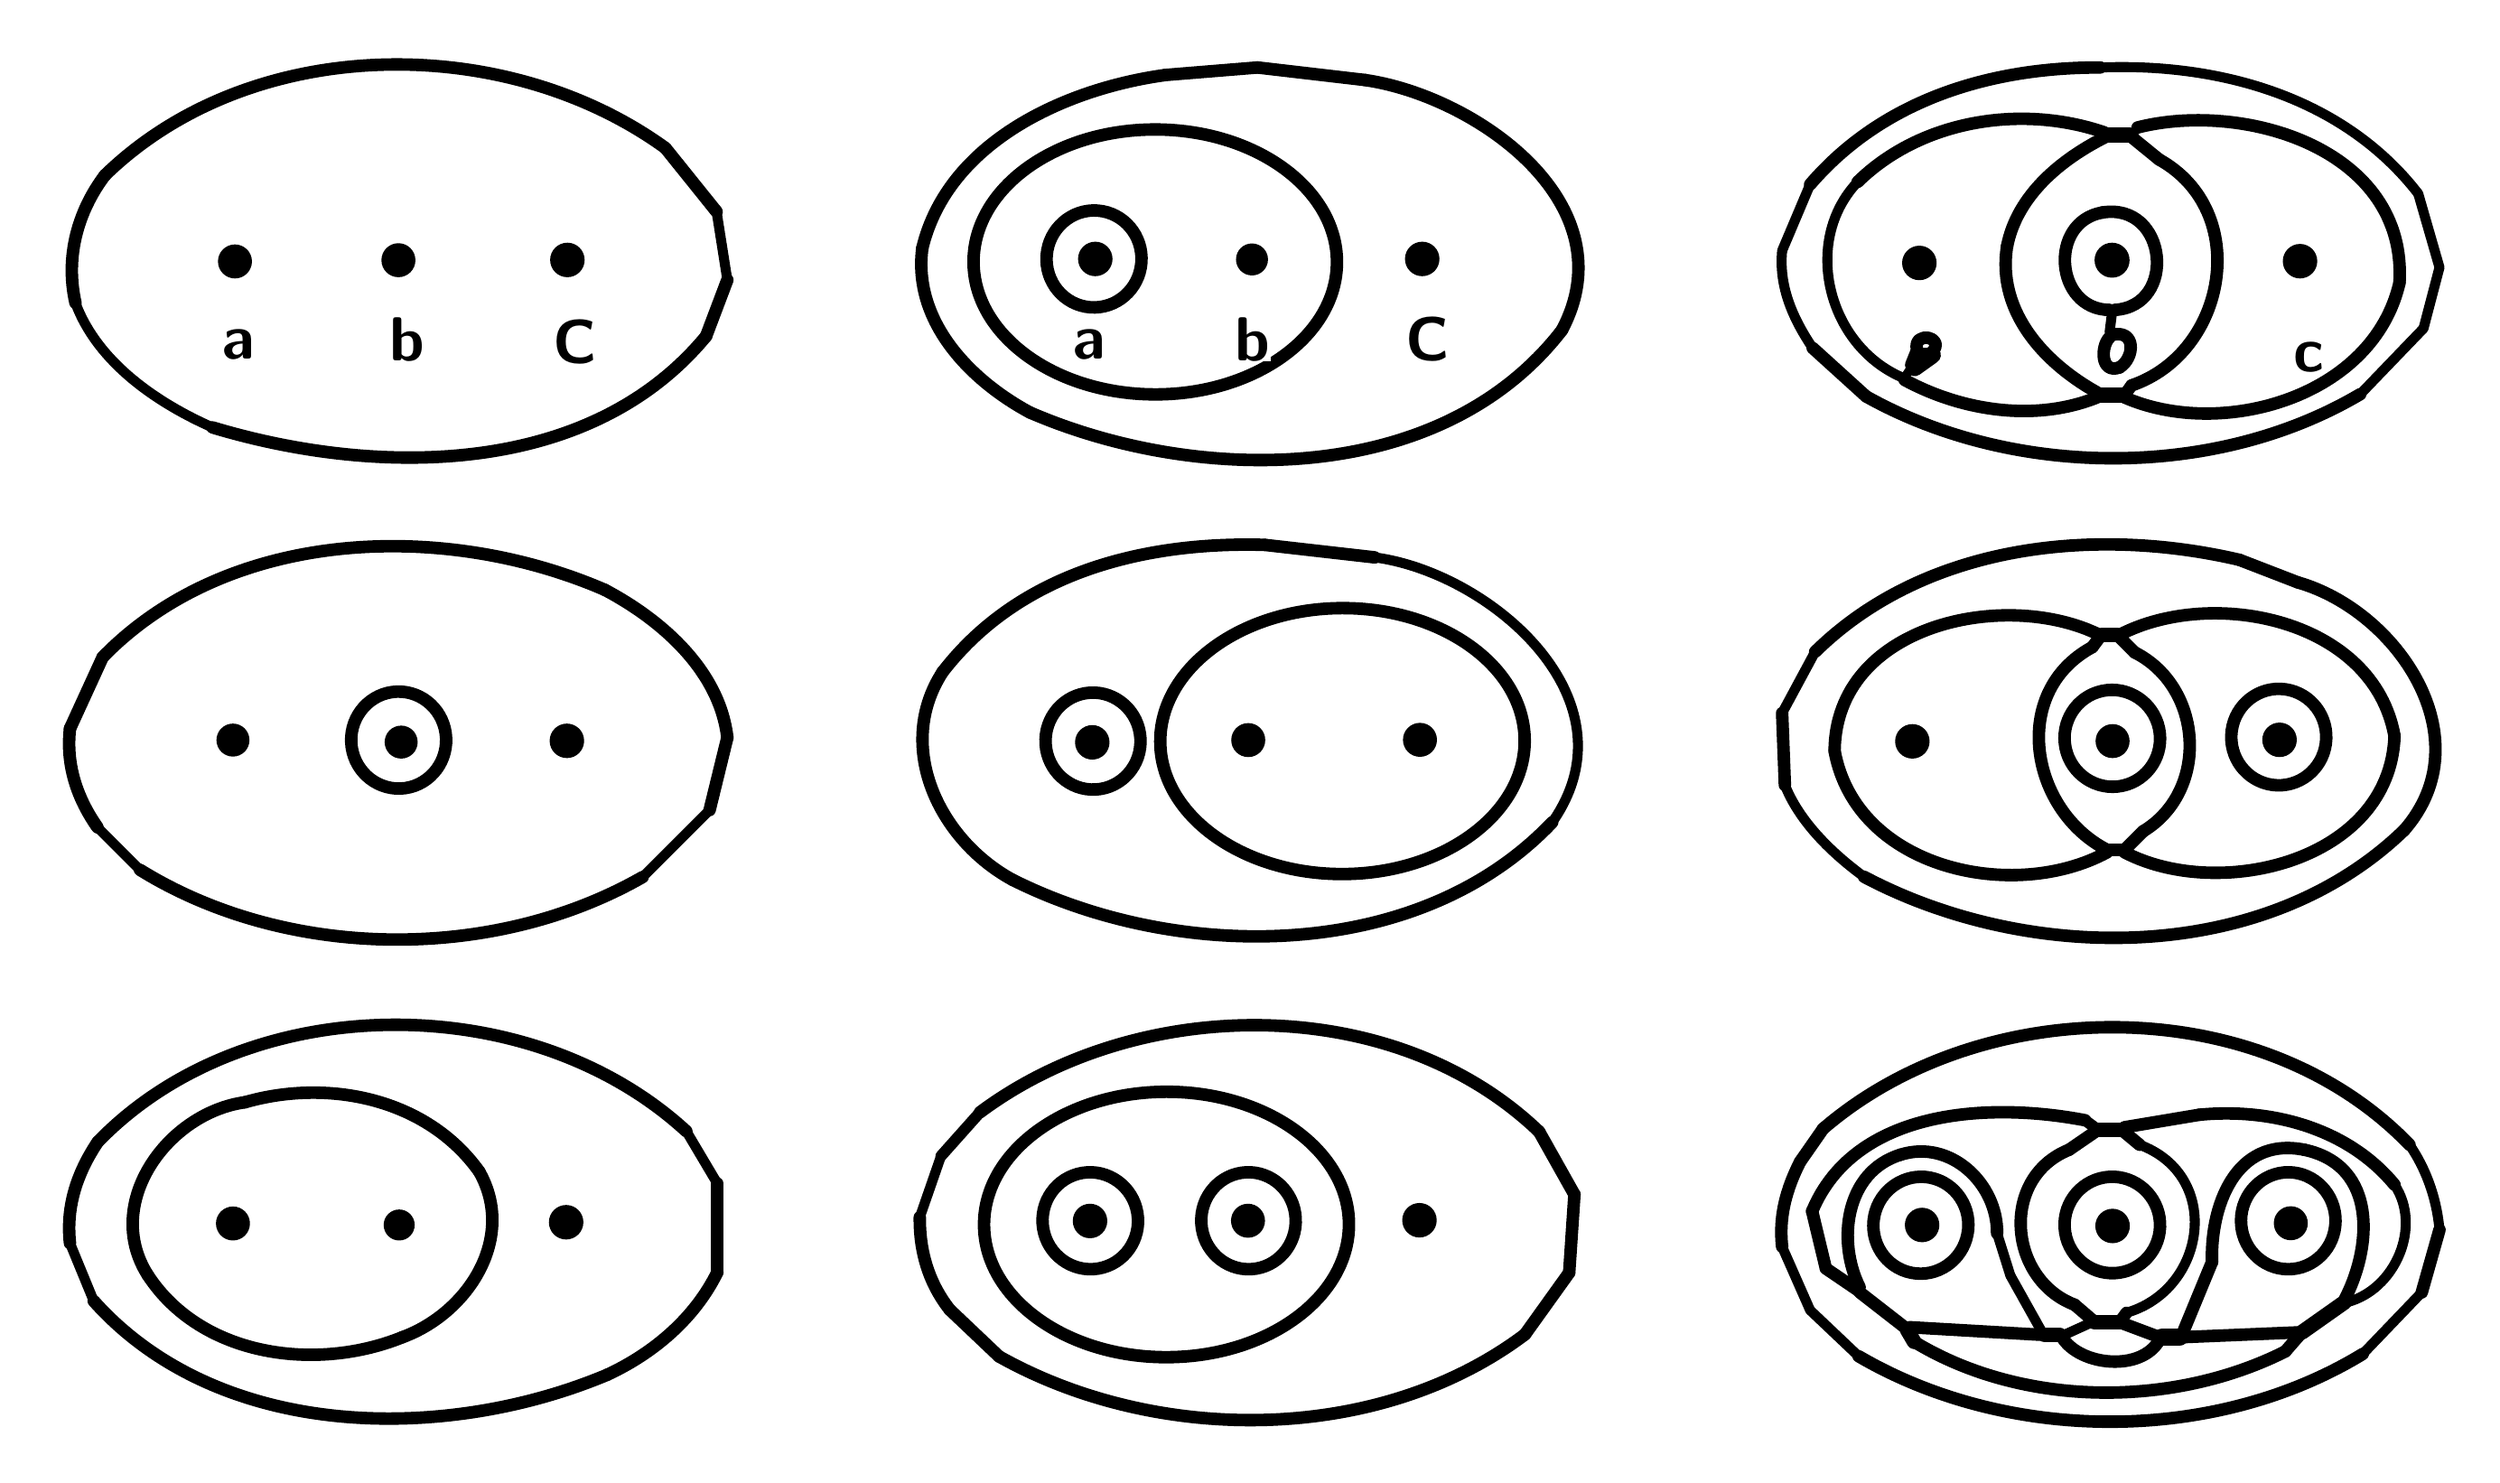
\begin{tikzpicture}[x=1pt, y=-1pt, line width=5.0pt, line cap=round, line join=round]

  %% ════ 填充区（prims2 的 fills）════

  %% ════ 直线段（prims2 的 strokes）════
  \draw[line width=5.0pt] (840.0,441.0) -- (869.9,436.0);
  \draw[line width=5.0pt] (840.0,443.0) -- (846.0,448.0);
  \draw[line width=4.9pt] (840.8,515.2) -- (838.0,519.0);
  \draw[line width=6.0pt] (831.0,244.0) -- (837.0,244.0);
  \draw[line width=4.0pt] (834.0,123.0) -- (835.0,115.0);
  \draw[line width=5.0pt] (733.0,506.0) -- (720.5,497.5);
  \draw[line width=5.0pt] (720.5,497.5) -- (715.0,474.6);
  \draw[line width=4.5pt] (824.2,438.2) -- (828.0,441.0);
  \draw[line width=5.0pt] (752.0,521.0) -- (734.0,507.0);
  \draw[line width=5.9pt] (753.0,522.0) -- (755.8,526.8);
  \draw[line width=5.0pt] (904.3,530.7) -- (911.0,523.0);
  \draw[line width=6.0pt] (833.0,44.0) -- (842.0,44.0);
  \draw[line width=4.0pt] (827.0,519.0) -- (816.0,524.0);
  \draw[line width=5.0pt] (875.0,494.9) -- (863.0,524.0);
  \draw[line width=3.5pt] (754.0,138.0) -- (752.0,141.0);
  \draw[line width=5.0pt] (754.0,521.0) -- (806.0,524.0);
  \draw[line width=4.9pt] (840.0,148.0) -- (842.8,144.2);
  \draw[line width=5.0pt] (853.8,53.8) -- (843.0,45.0);
  \draw[line width=5.0pt] (828.0,443.0) -- (817.8,450.0);
  \draw[line width=5.0pt] (820.0,512.0) -- (827.0,518.0);
  \draw[line width=6.0pt] (838.0,519.0) -- (828.0,519.0);
  \draw[line width=5.0pt] (838.0,519.0) -- (854.0,525.0);
  \draw[line width=6.0pt] (829.0,442.0) -- (839.0,442.0);
  \draw[line width=5.0pt] (830.0,245.0) -- (827.1,248.9);
  \draw[line width=4.0pt] (762.0,131.0) -- (758.0,131.0);
  \draw[line width=5.0pt] (863.0,525.0) -- (911.0,523.0);
  \draw[line width=6.0pt] (928.0,511.0) -- (911.0,523.0);
  \draw[line width=4.0pt] (789.0,483.4) -- (794.3,500.3);
  \draw[line width=4.0pt] (794.3,500.3) -- (807.0,523.0);
  \draw[line width=7.0pt] (763.0,132.0) -- (756.0,137.0);
  \draw[line width=6.0pt] (814.0,524.0) -- (808.0,524.0);
  \draw[line width=5.0pt] (839.0,330.0) -- (834.0,330.0);
  \draw[line width=5.7pt] (757.0,131.0) -- (755.0,136.0);
  \draw[line width=6.0pt] (830.0,148.0) -- (839.0,148.0);
  \draw[line width=5.0pt] (838.0,245.0) -- (844.0,251.0);
  \draw[line width=5.0pt] (847.4,322.6) -- (840.0,330.0);
  \draw[line width=7.0pt] (862.0,525.0) -- (855.0,525.0);
  \draw[line width=3.8pt] (845.2,41.0) -- (843.0,44.0);
  \draw[line width=4.0pt] (358.0,477.0) -- (366.5,452.5);
  \draw[line width=4.5pt] (366.5,452.5) -- (382.1,435.0);
  \draw[line width=5.0pt] (605.8,442.8) -- (619.9,467.9);
  \draw[line width=5.0pt] (619.9,467.9) -- (617.8,499.2);
  \draw[line width=5.0pt] (617.8,499.2) -- (600.1,523.9);
  \draw[line width=5.0pt] (389.7,532.7) -- (370.0,514.0);
  \draw[line width=5.0pt] (31.1,252.9) -- (18.0,281.5);
  \draw[line width=4.0pt] (29.0,321.0) -- (46.0,338.0);
  \draw[line width=4.0pt] (247.1,340.9) -- (273.9,314.1);
  \draw[line width=5.0pt] (273.9,314.1) -- (281.0,285.1);
  \draw[line width=5.0pt] (719.4,441.6) -- (710.2,454.8);
  \draw[line width=4.0pt] (703.0,488.8) -- (714.2,514.2);
  \draw[line width=4.0pt] (714.2,514.2) -- (733.6,532.6);
  \draw[line width=4.0pt] (935.3,531.7) -- (958.9,507.1);
  \draw[line width=5.0pt] (958.9,507.1) -- (966.0,482.0);
  \draw[line width=5.0pt] (256.2,49.2) -- (276.7,74.7);
  \draw[line width=4.0pt] (276.7,74.7) -- (281.0,102.0);
  \draw[line width=5.0pt] (281.0,102.0) -- (272.5,124.5);
  \draw[line width=5.0pt] (536.0,22.0) -- (493.1,17.0);
  \draw[line width=5.0pt] (493.1,17.0) -- (456.3,20.0);
  \draw[line width=5.0pt] (540.0,213.0) -- (496.0,208.0);
  \draw[line width=5.0pt] (277.0,499.0) -- (277.0,463.5);
  \draw[line width=4.0pt] (277.0,463.5) -- (264.6,442.6);
  \draw[line width=4.0pt] (18.0,487.4) -- (27.5,510.5);
  \draw[line width=4.0pt] (966.0,97.0) -- (957.5,67.5);
  \draw[line width=4.0pt] (714.2,63.8) -- (703.0,90.3);
  \draw[line width=5.0pt] (715.2,129.2) -- (736.6,148.6);
  \draw[line width=4.0pt] (934.3,147.7) -- (959.6,121.4);
  \draw[line width=4.0pt] (959.6,121.4) -- (966.0,97.0);
  \draw[line width=4.0pt] (716.2,250.8) -- (703.0,275.3);
  \draw[line width=5.0pt] (703.0,275.3) -- (704.1,304.1);
  \draw[line width=5.0pt] (909.3,223.0) -- (886.0,214.0);

  %% ════ 曲线（prims2 的 curves —— 三段式，坐标同为 (y,x)）════
  \draw[line width=5.0pt] (840.0,331.0) .. controls (877.6,350.7) and (946.1,334.8) .. (948.0,284.5);
  \draw[line width=5.0pt] (948.0,284.5) .. controls (939.6,237.6) and (875.1,224.7) .. (838.0,244.0);
  \draw[line width=5.0pt] (869.9,436.0) .. controls (898.5,433.2) and (929.3,441.3) .. (948.0,464.0);
  \draw[line width=4.0pt] (948.0,464.0) .. controls (959.2,480.7) and (948.3,506.0) .. (929.0,511.0);
  \draw[line width=4.0pt] (846.0,448.0) .. controls (879.4,460.4) and (872.7,506.0) .. (840.8,515.2);
  \draw[line width=5.0pt] (833.0,331.0) .. controls (795.8,351.2) and (732.7,337.9) .. (724.0,290.5);
  \draw[line width=5.0pt] (724.0,290.5) .. controls (724.3,239.9) and (792.2,225.3) .. (830.0,244.0);
  \draw[line width=5.0pt] (715.0,474.6) .. controls (732.1,433.6) and (785.7,430.8) .. (824.2,438.2);
  \draw[line width=5.0pt] (757.0,130.0) .. controls (755.0,122.2) and (768.7,124.5) .. (763.0,131.0);
  \draw[line width=5.0pt] (835.0,124.0) .. controls (844.6,121.6) and (844.2,133.2) .. (838.0,137.0);
  \draw[line width=5.0pt] (838.0,137.0) .. controls (830.3,139.8) and (830.4,128.5) .. (834.0,125.0);
  \draw[line width=5.0pt] (755.8,526.8) .. controls (799.1,553.1) and (859.2,553.4) .. (904.3,530.7);
  \draw[line width=5.0pt] (928.0,510.0) .. controls (938.9,489.3) and (941.6,456.3) .. (911.9,450.0);
  \draw[line width=5.0pt] (911.9,450.0) .. controls (884.1,444.5) and (874.3,473.0) .. (875.0,494.9);
  \draw[line width=5.0pt] (842.8,144.2) .. controls (881.1,131.1) and (891.0,74.5) .. (853.8,53.8);
  \draw[line width=5.0pt] (815.0,525.0) .. controls (822.0,536.5) and (846.8,539.1) .. (854.0,526.0);
  \draw[line width=5.0pt] (817.8,450.0) .. controls (790.0,461.2) and (793.4,501.9) .. (820.0,512.0);
  \draw[line width=5.0pt] (829.0,147.0) .. controls (808.0,135.3) and (788.8,114.7) .. (793.0,88.5);
  \draw[line width=5.0pt] (793.0,88.5) .. controls (797.0,68.2) and (814.4,53.9) .. (832.0,45.0);
  \draw[line width=5.0pt] (827.1,248.9) .. controls (793.7,267.0) and (802.3,314.3) .. (833.0,330.0);
  \draw[line width=5.0pt] (832.0,43.0) .. controls (798.9,31.6) and (758.6,37.9) .. (733.2,62.8);
  \draw[line width=4.0pt] (733.2,62.8) .. controls (710.7,86.5) and (721.2,128.2) .. (751.0,141.0);
  \draw[line width=5.0pt] (734.0,505.0) .. controls (724.9,486.8) and (728.1,458.9) .. (750.3,452.0);
  \draw[line width=5.0pt] (750.3,452.0) .. controls (770.6,445.6) and (789.2,463.8) .. (789.0,483.4);
  \draw[line width=5.0pt] (829.0,149.0) .. controls (804.4,158.9) and (775.0,154.5) .. (752.0,142.0);
  \draw[line width=5.0pt] (834.0,114.0) .. controls (812.0,113.8) and (809.4,78.7) .. (831.2,75.0);
  \draw[line width=5.0pt] (831.2,75.0) .. controls (857.2,70.9) and (861.3,112.5) .. (836.0,114.0);
  \draw[line width=5.0pt] (844.0,251.0) .. controls (871.5,264.8) and (874.1,306.5) .. (847.4,322.6);
  \draw[line width=5.0pt] (840.0,149.0) .. controls (878.8,166.0) and (939.5,149.0) .. (950.0,103.1);
  \draw[line width=5.0pt] (950.0,103.1) .. controls (953.1,49.5) and (887.7,30.2) .. (845.2,41.0);
  \draw[line width=5.0pt] (370.0,514.0) .. controls (361.6,503.4) and (357.8,490.6) .. (358.0,477.0);
  \draw[line width=5.0pt] (382.1,435.0) .. controls (445.1,388.0) and (547.3,386.6) .. (605.8,442.8);
  \draw[line width=5.0pt] (600.1,523.9) .. controls (541.5,568.0) and (452.6,568.0) .. (389.7,532.7);
  \draw[line width=5.0pt] (232.0,226.0) .. controls (168.6,198.5) and (82.1,200.6) .. (31.1,252.9);
  \draw[line width=5.0pt] (18.0,281.5) .. controls (16.3,296.3) and (21.0,309.6) .. (29.0,321.0);
  \draw[line width=5.0pt] (46.0,338.0) .. controls (104.6,374.3) and (187.3,375.1) .. (247.1,340.9);
  \draw[line width=5.0pt] (281.0,285.1) .. controls (277.9,258.3) and (254.7,238.0) .. (232.0,226.0);
  \draw[line width=4.0pt] (966.0,482.0) .. controls (964.9,469.8) and (960.9,458.1) .. (954.0,448.0);
  \draw[line width=5.0pt] (954.0,448.0) .. controls (894.3,386.0) and (783.0,386.8) .. (719.4,441.6);
  \draw[line width=5.0pt] (710.2,454.8) .. controls (704.9,465.3) and (701.6,476.2) .. (703.0,488.8);
  \draw[line width=5.0pt] (733.6,532.6) .. controls (793.1,567.4) and (875.8,568.0) .. (935.3,531.7);
  \draw[line width=4.0pt] (75.0,161.0) .. controls (52.8,151.2) and (29.0,135.0) .. (20.2,111.2);
  \draw[line width=5.0pt] (20.2,111.2) .. controls (16.0,92.8) and (21.1,74.5) .. (32.0,60.1);
  \draw[line width=5.0pt] (32.0,60.1) .. controls (90.4,3.3) and (192.0,2.7) .. (256.2,49.2);
  \draw[line width=5.0pt] (272.5,124.5) .. controls (225.3,181.6) and (139.7,180.5) .. (75.0,161.0);
  \draw[line width=5.0pt] (456.3,20.0) .. controls (416.7,25.4) and (369.3,46.5) .. (359.0,89.3);
  \draw[line width=5.0pt] (359.0,89.3) .. controls (355.2,118.6) and (378.1,142.1) .. (402.0,155.0);
  \draw[line width=5.0pt] (402.0,155.0) .. controls (468.8,183.9) and (566.2,185.1) .. (614.9,122.1);
  \draw[line width=5.0pt] (614.9,122.1) .. controls (641.9,71.3) and (580.1,28.3) .. (536.0,22.0);
  \draw[line width=5.0pt] (496.0,208.0) .. controls (447.4,206.6) and (397.7,219.2) .. (367.1,258.9);
  \draw[line width=5.0pt] (367.1,258.9) .. controls (347.8,288.7) and (365.7,326.0) .. (395.1,342.0);
  \draw[line width=5.0pt] (395.1,342.0) .. controls (461.0,375.0) and (557.3,375.6) .. (611.0,319.0);
  \draw[line width=4.0pt] (611.0,319.0) .. controls (645.5,269.9) and (586.1,219.1) .. (540.0,213.0);
  \draw[line width=5.0pt] (233.0,540.0) .. controls (251.5,531.4) and (268.0,517.4) .. (277.0,499.0);
  \draw[line width=5.0pt] (264.6,442.6) .. controls (201.9,384.9) and (88.6,385.3) .. (29.1,446.9);
  \draw[line width=5.0pt] (29.1,446.9) .. controls (21.2,458.7) and (16.3,472.2) .. (18.0,487.4);
  \draw[line width=5.0pt] (27.5,510.5) .. controls (77.7,566.7) and (168.3,567.2) .. (233.0,540.0);
  \draw[line width=4.0pt] (957.5,67.5) .. controls (927.3,28.5) and (877.4,15.1) .. (830.3,17.0);
  \draw[line width=5.0pt] (830.3,17.0) .. controls (786.6,16.9) and (743.5,29.7) .. (714.2,63.8);
  \draw[line width=4.0pt] (703.0,90.3) .. controls (701.6,105.0) and (707.5,117.7) .. (715.2,129.2);
  \draw[line width=5.0pt] (736.6,148.6) .. controls (795.2,181.4) and (876.1,182.1) .. (934.3,147.7);
  \draw[line width=5.0pt] (88.0,431.0) .. controls (121.0,421.5) and (160.6,429.2) .. (181.7,458.7);
  \draw[line width=5.0pt] (181.7,458.7) .. controls (196.8,485.2) and (177.2,515.4) .. (151.0,525.0);
  \draw[line width=5.0pt] (151.0,525.0) .. controls (117.0,538.8) and (70.7,533.2) .. (49.1,500.1);
  \draw[line width=5.0pt] (49.1,500.1) .. controls (30.8,471.2) and (57.3,435.2) .. (88.0,431.0);
  \draw[line width=5.0pt] (886.0,214.0) .. controls (827.8,200.4) and (760.0,207.7) .. (716.2,250.8);
  \draw[line width=4.0pt] (704.1,304.1) .. controls (709.9,318.7) and (722.7,331.2) .. (735.8,340.8);
  \draw[line width=5.0pt] (735.8,340.8) .. controls (801.3,375.5) and (895.6,376.6) .. (951.9,322.1);
  \draw[line width=5.0pt] (951.9,322.1) .. controls (983.7,285.7) and (949.3,234.4) .. (909.3,223.0);

  %% ════ 圆 / 椭圆（probe 精测）════
  \draw[rotate around={90.1:(456.7,479.9)}] (456.7,479.9) ellipse (53.1 and 73.0);
  \draw[rotate around={90.2:(527.1,286.5)}] (527.1,286.5) ellipse (53.2 and 72.9);
  \draw[rotate around={89.9:(452.2,94.8)}] (452.2,94.8) ellipse (53.0 and 72.7);
  \draw[rotate around={12.1:(835.1,285.4)}] (835.1,285.4) ellipse (19.1 and 19.4);
  \draw[rotate around={179.4:(905.5,478.4)}] (905.5,478.4) ellipse (18.9 and 19.4);
  \draw[rotate around={3.4:(427.3,286.5)}] (427.3,286.5) ellipse (19.0 and 19.4);
  \draw[rotate around={177.9:(901.7,284.9)}] (901.7,284.9) ellipse (19.0 and 19.3);
  \draw[rotate around={9.0:(835.1,480.1)}] (835.1,480.1) ellipse (19.1 and 19.3);
  \draw[rotate around={168.8:(758.5,480.2)}] (758.5,480.2) ellipse (19.0 and 19.4);
  \draw[rotate around={9.3:(426.2,478.4)}] (426.2,478.4) ellipse (19.1 and 19.4);
  \draw[rotate around={175.5:(427.7,93.6)}] (427.7,93.6) ellipse (19.0 and 19.4);
  \draw[rotate around={3.3:(489.5,478.4)}] (489.5,478.4) ellipse (18.9 and 19.4);
  \draw[rotate around={2.2:(149.5,286.1)}] (149.5,286.1) ellipse (19.0 and 19.4);

  %% ════ 实心点 ════
  \fill (428.2,93.6) circle (6.9);
  \fill (559.0,93.6) circle (6.9);
  \fill (84.0,94.6) circle (6.8);
  \fill (149.4,94.1) circle (6.8);
  \fill (217.0,94.0) circle (6.9);
  \fill (835.0,94.1) circle (7.0);
  \fill (910.2,94.5) circle (6.9);
  \fill (490.9,93.8) circle (6.4);
  \fill (757.9,95.2) circle (6.9);
  \fill (216.8,286.4) circle (6.9);
  \fill (489.4,286.1) circle (6.8);
  \fill (558.1,286.0) circle (6.8);
  \fill (755.1,286.6) circle (6.9);
  \fill (835.2,286.5) circle (6.8);
  \fill (902.0,286.0) circle (6.9);
  \fill (83.2,286.1) circle (6.6);
  \fill (427.0,287.0) circle (6.9);
  \fill (150.5,286.9) circle (6.6);
  \fill (216.5,479.0) circle (6.9);
  \fill (426.1,478.5) circle (6.9);
  \fill (489.3,478.4) circle (6.8);
  \fill (557.9,478.2) circle (6.9);
  \fill (83.2,479.5) circle (6.8);
  \fill (906.5,479.4) circle (6.8);
  \fill (759.0,480.1) circle (6.9);
  \fill (835.2,480.5) circle (6.9);
  \fill (149.7,480.1) circle (6.2);

  %% ════ 标签（probe 直接给的 \node 行）════
  %% ⚠ 全部补了 fill=white：文字在最上层，否则与曲线交叉干扰
     \node[anchor=center,inner sep=0pt,fill=white,font=\fontsize{30.7}{38.3}\selectfont] at (152.8,125.8) {\textsf{\textbf{\textit{b}}}};   % box(143,113,17,23)
     \node[anchor=center,inner sep=0pt,fill=white,font=\fontsize{31.6}{39.5}\selectfont] at (491.3,125.8) {\textsf{\textbf{\textit{b}}}};   % box(481,113,18,23)
     \node[anchor=center,inner sep=0pt,fill=white,font=\fontsize{23.4}{29.3}\selectfont] at (561.1,125.7) {\textsf{\textbf{\textit{C}}}};   % box(553,117,15,17)
     \node[anchor=center,inner sep=0pt,fill=white,font=\fontsize{33.0}{41.2}\selectfont] at (85.6,128.1) {\textsf{\textbf{\textit{a}}}};   % box(76,118,17,17)
     \node[anchor=center,inner sep=0pt,fill=white,font=\fontsize{23.4}{29.3}\selectfont] at (220.1,126.7) {\textsf{\textbf{\textit{C}}}};   % box(212,118,15,17)
     \node[anchor=center,inner sep=0pt,fill=white,font=\fontsize{32.0}{40.0}\selectfont] at (426.1,128.1) {\textsf{\textbf{\textit{a}}}};   % box(417,118,16,17)
     \node[anchor=center,inner sep=0pt,fill=white,font=\fontsize{31.4}{39.3}\selectfont] at (913.8,133.1) {\textsf{\textbf{\textit{c}}}};   % box(905,123,16,17)

  % 钉死画布：否则超出的图元/控制点会把页面撑大，1:1 回比就失准
  \pgfresetboundingbox
  \path[use as bounding box] (0,0) rectangle (980,573);
\end{tikzpicture}
\end{document}

% ⚠ 待核清单（probe 拿不准，人眼过一遍）：
%   · 未识别/跳过：⑤ 跳过/未识别的字形
%   · 未识别/跳过：box(407,72,43,45)
%   · 未识别/跳过：box(405,457,44,44)
%   · 未识别/跳过：box(469,457,43,44)
